\chapter{FPGA} % Main chapter title
\label{FPGA} % For referencing the chapter elsewhere, use \ref{Chapter1} 

\section{Einleitung}
Ein FPGA (Field Programmable Gate Array) ist ein integrierter Schaltkreis, in den eine beliebige logische Schaltung programmiert werden kann.

Die meisten FPGA's basieren auf mehrfach beschreibbarem (EEPROM-) Speicher. Dadurch kann die umgesetzte Logik eines FPGA's beliebig oft durch das Laden einer Konfigurationsdatei geändert werden. Sie eignen sich daher insbesondere für die Prototyping- und Testphase von Hardwareprojekten, da sie kostengünstig und schnell neu konfiguriert werden können. \cite[S. 8]{SynthesisFPGA}

\section{Technik}
\paragraph{Configurable Logic Blocks.} FPGA's bestehen aus einem zweidimensionalen Array von programmierbaren Blöcken, den \emph{Configurable Logic Blocks} (CLB). \cite[S. 11]{Chu} Der genaue Aufbau ist dabei herstellerabhängig, sie bestehen aber mindestens aus einem Look-Up Table (LUT) und einem Flipflop. \cite[S. 8]{SynthesisFPGA}

\begin{figure} [ht]
  \centering
  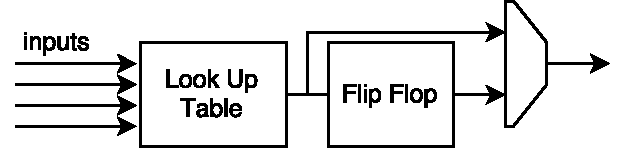
\includegraphics[width=0.5\textwidth]{Figures/clb}
  \caption{Aufbau eines simplen Configurable Logic Block.}
  \label{fig:clb}
\end{figure}


\paragraph{Look-Up Tables.} Look-Up Tables haben $n$ Eingänge (meistens zwischen 4 und 6) und einen Ausgang. Sie sind so konfigurierbar, dass sie eine beliebige Binärfunktion umsetzen. Zu diesem Zweck enthält jede LUT $2^n$ Speicherzellen, in denen die Werte für jede beliebige Eingangssignalkombination abgelegt werden können. Sie sind so verschaltet, dass eine bestimmte Eingangskombination zur Ausgabe des Wertes der dazugehörigen Speicherzelle führt. \cite[S. 12f.]{Chu} Durch Neubelegung dieser Speicherzellen kann die umgesetzte Logik des FPGA's beliebig verändert werden. 

\paragraph{Flipflops.} Durch den fest verbauten D-Flipflop kann die Ausgabe des Logikblocks nicht nur direkt weitergegeben, sondern auch zwischengespeichert werden. Dadurch lassen sich rückgekoppelte Logiken (Schaltwerke) realisieren. \cite[S. 13]{Chu}

\paragraph{Verbindungen.} Die einzelnen CLB's sind wiederum mit konfigurierbaren Verbindungen verdrahtet. Dafür liegt zwischen den Blöcken ein Gitter aus Leitungen, an deren Kreuzungspunkten die Signalverteilung mitteils eines programmierbaren Schalters beliebig konfiguriert werden kann. \cite[S. 12]{Chu}

\section{Verwendete Hardware}
Für dieses Projekt wurde das \emph{Nexys 4}-Board mit einem Xilinx \emph{Artix-7}-FPGA verwendet. Dieser enthält $101440$ Logic Cells, die in $15850$ Logic Slices organisiert sind. Diese sind wiederum aus jeweils vier LUT's mit sechs Inputs und acht Flipflops aufgebaut. Der FPGA erlaubt die Implementierung von bis zu $1188$ kB Distributed RAM (durch die Logikbausteine implementierter RAM). Das Board wird mit einem internen 100Mhz Takt versorgt. \cite{Artix}